\chapter{Secret Storage as a Service}
\label{chap:ssaas}

As discussed in Chapter~\ref{chap:challenges}, the reliance on third
parties inherent to many popular use cases poses a number of privacy
and security related challenges. Fortunately, cryptographic techniques
including encryption and authentication provide the necessary
primitives for building a systems that increases the security and
privacy of users by reducing their exposure to third party trust
abuses. Such mechanisms also provide additional security beyond third
party risk: e.g. by ensuring that systems such as mobile devices remain
secure even if lost or stolen. Unfortunately, cryptography is not
merely ``magic fairy dust'' that developers can sprinkle on any
security or privacy problem to make it
disappear~\cite{smith2003}. Effectively using cryptographic technique
to secure user data involves ensuring that cryptography-based solution
are designed in both a secure and a usable manner.

One of the critical components of building secure and usable
cryptographic data security solutions lies in providing secure and
flexible key management systems that can be leveraged to store the
cryptographic keys associated with such systems. The failure of
traditional cryptographic systems to account for key management has
led many such systems to be unusable, insecure, and/or ill-adapted to
modern use cases. Such key management systems are but one facet of the
larger secret storage problem: the need to use to store a range of
secrets from passwords to personal data in a manner that is both
secure and usable.

This chapter discusses the Secret Storage as a Service (SSaaS) model:
a service oriented secret storage method designed to provide users
with the necessary tools for managing secrets in a manner that allows
for a range of use cases while also avoiding the need to place high
degrees of trust in any single third party.

\section{Architecture}
\label{chap:ssaas:arch}

Secret Storage as a Service (SSaaS) is a service oriented architecture
where users utilize dedicated Secret Storage Providers (SSPs) in
addition to traditional Feature Providers (FPs) such as Amazon,
Dropbox, Gmail, or Facebook. An SSP is tasked with the storage of and
access control to a variety of user secrets from cryptographic keys to
personal data. FPs, on the other hand are limited to storing less
sensitive information such as cryptographically protected
data\footnote{At least in the normative case. There are also SSP use
  cases that involve no FP at all: e.g. storing user passwords.}, the
keys for which reside with one or more SSPs. This allows SSPs to be
selected on the basis of their trustworthiness while traditional
feature providers can be selected on the basis of their feature
sets. The SSaaS model differs from the traditional cloud model by
allowing users to distribute trust across multiple third parties (or
no third parties at all), ensuring that no single entity need be fully
trusted, while still enabling many popular use cases.

\subsection{Stored Secrets}

In the SSaaS model, what kind of secrets does a user store with an
SSP? Users should be able to store arbitrary data with any SSP,
allowing open-ended secret storage based applications. That said, the
SSP model works best when secrets stored are not themselves inherently
sensitive or revealing. This property helps to mitigate the amount a
user must trust each SSP. Thus, storing secrets like cryptographic
keys that alone reveal no private user data is generally preferable to
storing privacy revealing secrets like social security numbers,
etc. The decision of what to store with each SSP, however, is left up
to each user and application to maximize the flexibility of the SSaaS
model. Chapter~\ref{chap:apps} explores various types of secret
storage applications.

Another consideration related to what secrets to store with an SSP is
size. It is reasonable to predict that SSP-based storage will sell at
a premium price vs more traditional cloud storage options like Amazon
S3~\cite{amazon-s3}. This is due to the difference in priorities
between Secret Storage and generic cloud storage. An SSP is primarily
concerned with safeguarding user secrets and faithfully implementing a
user's access control specifications for each secret. These priorities
may very well incur additional costs not present in more traditional
cloud storage environments: e.g. the need to locate data centers in
specific legal jurisdictions, a greater emphasis of resistance to
compelled violations via legal representation, etc. Thus, it may be
desirable for the user to minimize the amount of data stored with an
SSP as a cost optimization: again making use cases such as storing
relatively small cryptographic keys with an SSP while storing the
marge larger encrypted data with a more traditional provider
desirable.\footnote{For these reasons, storing cryptographic keys with
  an SSP is a common enough use case that some SSPs may specifically
  optimize for it. Such ``Key Storage as a Service'' (KSaaS) SSPs
  represent a subset of the general SSaaS model.}

\subsection{Secret Storage Providers}

In the SSaaS model, SSPs will offer a standard set of features. These
include a standardized storage interface, access control primitives,
and auditing capabilities. These features provide the basis of
building privacy-preserving SSaaS-backed applications.

\subsubsection{Secret Storage}

At its core, an SSP provider is offering a key:value data storage
model. Each secret is tagged with a key: a unique identifier,
potentially a UUID~\cite{leach2005} or similar unique ID standard. The
value associated with each ID is then the user's secret itself, be it
a cryptographic key, personal user data, or arbitrary secret
value. Users are able to query each SSP for the value associated with
a given ID.

Optionally, SSPs may provide versioning of each id:secret pair. This
may be desirable for use cases where the user wishes to share data
with other users while maintaining the ability to revoke shared access
to future versions of a data set. Such ``lazy
revocation''~\cite{kallahalla2003} capabilities can be built atop
versioning schemes that maintain access control information on a
per-version basis.

Each SSP will expose its key-value secret store via a RESTful
HTTPS-based API\footnote{The exact mechanism powering the API
  interface is not relevant to the SSaaS model as a whole, but given
  the ubiquity and simplicity of RESTful designs, it seems a
  reasonable choice for an SSaaS standard.}. The ubiquity of RESTful
interfaces in modern applications ensures that such an interface will
allow simple communication between a client and the SSP across a wide
variety of platforms. This interface will expose create, read, modify,
delete semantics similar to most existing key:value stores. In fact,
it is likely that most SSP implementations will use an off-the-shelf
key-value store as the backend for storing user secrets. I intend for
SSPs to utilize a standard API in order to allow users to interact with
multiple SSPs and transfer their secrets between SSPs.

\subsubsection{Access Control}

The SSP data model associates an access control specification with
each id:secret pair (or in a versioned system, with each
id:version:secret set). This specification governs the manner in which
a given secret can be accessed. Such specification will be provided
and controlled by creator of each secret, potentially delegating such
control to other users as well. The SSP is in charge of faithfully
enforcing the access control specification.

An access control specification dictates who can create, access,
modify, or delete each secret. It contains information regarding both
authentication (how a user proves they are who they claim to be) as
well as authorization (what permissions each authenticated user is
granted). It is desirable for SSPs to offer a standard access control
framework in order to promote interoperability between multiple SSPs.

It is important that the SSP access control model remain
flexible. Since an SSP may be asked to store a variety of secrets in
support of a range of use cases, the access control model must be
expressive enough to avoid artificially limiting the user to specific
use cases or secrets. For example, one use case might require a single
user to satisfy multiple challenges in order to gain access to a
highly sensitive secret while another might require autonomous access
to a secret used by an automated processes (e.g. a secure backup
system), potentially limited to systems possessing a special token or
to specific times of day.

In addition to the key:value storage API operations discussed
previously, an SSP will also expose API endpoints for manipulating the
access control parameters associated with each secret as part if the
standard API. This interface will allow users to update access control
information to allow data sharing with other users, revoke prior
shared access, etc. This interface will, in turn, require it is own
access control specification to ensure that only approved
modifications can be made to any secret's access control rules.

\subsubsection{Auditing}

In addition to access control, each SSP should provide auditing
information related to the manner in which each id:secret pair is
accessed or modified. This information is useful to the user in order
to provide additional transparency into the manner in which secrets
are utilized. This auditing can be as simple as basic logging of all
secret access or as complex as a system that automatically analyzes
access patterns to try to detect anomalies that might indicate
potential trust violations.

Auditing information is useful to users for several reasons. In the
event that user data or secrets are ever unintentionally leaked or
compromised, audit information can provide a valuable indication of
the scope of the damage. Furthermore, auditing plays an important role
in allowing users to understand the semantics of access revocations:
since it is unfeasible to revoke access to data another user has
already read (and potentially copied out-of-band), audit information
provides a user with the scope of potentially revocable outstanding
authorization allowances. E.g. if User A shares a secret with User B
by granting them read access via their SSP, but then decides they'd
rather revoke that access, User A can check the audit logs to
determine if User B has already accessed the shared secret and thus
whether or not guaranteed revocation is even possible.

As with the other SSP core functions, an SSP's auditing capabilities
will be exposed via the SSP API to allow client applications to
leverage audit data. Likewise, audit API functions will need their own
set of access control specifications in order to control who has
access to audit information or the ability to delete that
information. As before, standardizing this interface is desirable from
an SSP interoperability standpoint.

It may also be desirable for SSPs to employ some form of
publicly-verifiable audit trail, similar to the concepts discussed
in~\cite{blaze1996} or~\cite{laurie2013}. Alternatively, such systems
might be constructed using block-chain-based primitives such as those
available in the BitCoin crypto-currency
network~\cite{Nakamoto2008}. Such public audit logs might provide more
robust variants of the ``warrant cannery'' concept that has recently
become popular amongst a range of third party services providers as a
counter measure against secret compelled data
requests~\cite{eff-canary}.

SSP audit logs could also be interfaced with third-party analysis
engines (e.g.~\cite{logrythm} or~\cite{splunk}) in order to spot
abnormal access patterns or other security-related anomalies. The
logically-centralized nature of SSPs make them a desirable point at
which to audit and detect unauthorized access requests for user data
via such mechanisms.

\subsection{Clients}

While SSPs form one half of the SSaaS architecture, the other half is
formed by clients connecting to and leveraging data from
SSPs. Chapter~\ref{chap:apps} discusses potential SSaaS use cases and
applications in detail. This section outline some of the basics of
SSaaS client deign and operation.

An SSaaS client is any system designed to connect to and utilize a
Secret Storage Provider. Clients communicate with one or more SSPs via
the SSP API. Clients can store and retrieve secrets with each SSP,
manage secret access control settings, and retrieve secret access
audit info. Examples of SSaaS client applications include encrypted
file systems, secure communication systems, dedicated
crypto-processing systems, etc. Any system that stands to benefit from
offloading secret storage and management to a dedicated service is a
good candidate for integration into an SSaaS architecture. Such
benefits might be derived either from the logically centralized nature
of an SSP (e.g. for the purpose of accessing secrets from multiple
devices or for sharing them with multiple users) or from the simple
desire to avoid implementing a full secret management and access
control stack locally,

In the simplest case, each SSaaS client communicates with a single
upstream SSP via a standard protocol. The standardized protocol allows
the end user to specify which SSP they wish to use, and to change SSPs
as desired. The downside to such a single SSP arrangements lies in the
fact that storing each secret with only one SSP raises both trust and
availability concerns (the details of which are discussed below). To
overcome such concerns, it is important for each SSaaS client to be
able interact with multiple SSPs, sharding each secret across multiple
SSPs and increasing reliability while reducing trust in the
process. Such multi-SSP arrangements, however, raise client side
management issues. How are access control rules managed across SSPs?
How does the client keep multiple SSPs in sync? Potential answers to
these questions are provided by the Tutamen work presented in
Chapter~\ref{chap:tutamen}.

\section{Economics}
\label{chap:ssaas:economics}

Part of the the argument in favor of the SSaaS model is
economics. Today, users primarily select cloud services on the basis
of their features. When they pay for these services, they're primarily
paying to support the core features such services provide. Privacy and
security, while potential concerns, are at best secondary
goals. Furthermore, on many free cloud services, the ability to
harvest user data is the basis of the service provider's business
model. As discussed in Section~\ref{chap:trust:survey}, these
situations create a number of perverse incentives in terms of a
traditional feature provider's goals with respect to user security and
privacy~\cite{anderson2001}. In the first case, the feature provider
simply does not prioritize user security since that is not the primary
basis on which users are choosing to pay for a service. In the second
case, a feature provider actively works to subvert user security and
privacy in order to further leverage user data to generate income.

The SSaaS model aims to rectify these issues by introducing SSP actors
whose primary goal is the protection of user secrets and from whom
users purchase secret storage services on the basis of security and
privacy guarantees. Thus, SSaaS's ability to separate secret storage
duties from feature provider duties allows users to purchase each
service on the basis of its associated merits, avoiding the issues
associated with putting features in direct competition with security
and privacy: a competition that security and privacy have historically
lost. Given such separation, independent markets can form around
feature provision and secret protection, optimized for the respective
priorities of each field.

Beyond the removal of perverse incentives brought about by the
separation of SSPs and FPs, it is also desirable to encourage a
competitive market amongst multiple SSP providers. In order to achieve
such a market, it's necessary to standardize on a single
inter-compatible SSaaS protocol. Such a standard protocol gives users
a high degree of mobility between competing SSPs providers, avoiding
vendor lock-in. This mobility, in turn, increases the competitive
pressures between providers. In short, the aim of an SSaaS ecosystem
is to make security and privacy tradable commodities, and to leverage
market powers to price and improve both. A competitive market for
secret storage has a number of security and privacy enhancing
benefits:

\begin{packed_desc}
\item[Reputation:] If users can easily switch between SSPs, it forces
  SSPs to compete on the basis of their security and privacy
  preserving reputations. SSPs who can do a superior job avoiding the
  trust violations discussed in Chapter~\ref{chap:trust} can attract
  more users and/or command a higher price for their services. Since a
  SSP's reputation is tied solely to their ability to faithfully
  protect user secrets, they will not be able to ``iron over'' any
  privacy-related reputation failings with superior end user feature
  sets -- a practice employed by many traditional feature
  providers~\footnote{As an example, consider Facebook's numerous
    trust violations~\cite{goel2014, lomas2014, tsukayama2014} and the
    fact that such violations have had no noticeable impact on the
    number of people using Facebook~\cite{foster2014}. An SSP would
    enjoy no such network benefit from providing additional services
    beyond secret storage were they to violate user's trust; instead,
    users would simply switch to a new SSP.}.
\item[Multiple Providers:] A healthy ecosystem of competing SSPs will
  allow users to select from multiple independent providers over which
  they may shard a single secret. Such sharding (discussed below)
  provides a number of benefits over relying on a single SSP, from
  trust reduction to data redundancy.
\item[Cost:] As in other competitive markets, having a number of
  competing providers will allow the user to select a provider that
  offers the best combination of cost and service.
\end{packed_desc}

The SSaaS model also provides business benefits related to liability
and insurance. Having a dedicated entity in charge of protecting user
secrets (and by proxy, any other data protected by those secrets)
simplifies the process of evaluating risk and liability related to the
protection of sensitive data. SSPs could provide insurance polices to
their users to indemnify them against any loss caused by a trust
violation on the part of the SSP. Likewise, SSPs would underwrite such
user-facing insurance polices with their own insurance polices
provided by independent third party insurers. These insurers would
need to perform independent audits\footnote{Potentially similar to the
  audit model used by Certificate Authorities in the PKI system,
  e.g.~\cite{hall-caaudit, mozilla-capolicy}.} of SSP infrastructure
and polices in order to evaluate trust violation risk. Such audits
further incentivizes SSPs to design their services specifically for
the avoidance of such trust violations. Such ``cyber'' insurance
benefits are not as readily available in the mixed trust + feature
cloud ecosystem of today since it is far harder to evaluate the
privacy violation risk of a company whose primary objectives are more
complex then secret storage alone~\cite{ciab2015}. The increasing
regulation of user privacy rights and the penalties associated with
violating user privacy further incentive a system where privacy and
security are severable properties that can be independently regulated,
evaluated, and indemnified -- unconnected to the user-facing feature
set of a given third party service. These ideas are discussed in more
depth in Chapter~\ref{chap:policy}

Likewise, SSaaS provides compliance benefits to users storing highly
regulated data by shifting compliance burdens from FPs to
SSPs. Instead of having to individually verify that each FP cloud
service meets the requirements of a specific data storage regulation,
a user could instead simply make sure that their SSP meets the
necessary requirements. Once certified, a single SSP could be reused
with multiple FPs without having to undergo further compliance
verification. SSPs might even proactively obtain specific compliance
certifications to make it easy for their users to comply with specific
regulations, regardless of which feature-providing cloud service a
user wishes to store encrypted data with. Such practices would likely
prove beneficial in highly-regulated fields such as health care
(e.g. requiring HIPPA~\cite{hippa} compliance), education
(e.g. requiring FERPA~\cite{ferpa} compliance), and online payment
processing (e.g. requiring PCI DSS~\cite{pcidss} compliance).

\section{Security and Trust}
\label{chap:ssaas:trust}

As mentioned in Chapter~\ref{chap:trust}, use cases that involve
splitting user data into cryptographically protected core data and the
associated cryptographic keys (i.e. secrets) and storing each with
separate providers inherently decreases the level of trust that any
single provider must be afforded. If, however, a user wishes to store
unencrypted data directly with an SSP,\footnote{Potentially because a
  given use case can't easily be split into encrypted data and
  encryption keys.} they must place a higher degree of trust in an
SSP. In the split encrypted data + cryptographic secrets use case, the
user must only trust the SSP with the storage (\emph{S}) and metadata
(\emph{M}) capabilities, the same capabilities with which they must
trust the FP. But in the case where an SSP directly stores raw user
data, they must expand their capability profile to also include the
access (\emph{R} ) and manipulation (\emph{W}) capabilities. Are SSPs
any more worthy (i.e. less likely to violate) this increased level of
trust than a traditional FP?

Even in such a ``heightened degree of trust'' scenario, SSPs would
appear less likely to violate user trust than traditional FPs. As
outlined in \S~\ref{chap:ssaas:economics}, SSPs have economic
incentives well aligned with upholding a user's trust where as
traditional FPs often have economic incentives in direct conflict with
upholding user trust. This fact alone decreases an SSP's likelihood of
trust violation by disincentivizing implicit violations
(\emph{P}-type) and putting a higher premium on avoiding unintentional
(\emph{U}-type), insider (\emph{I}-type), and outsider (\emph{O}-type)
violations.

\begin{figure}[t]
  \centering
  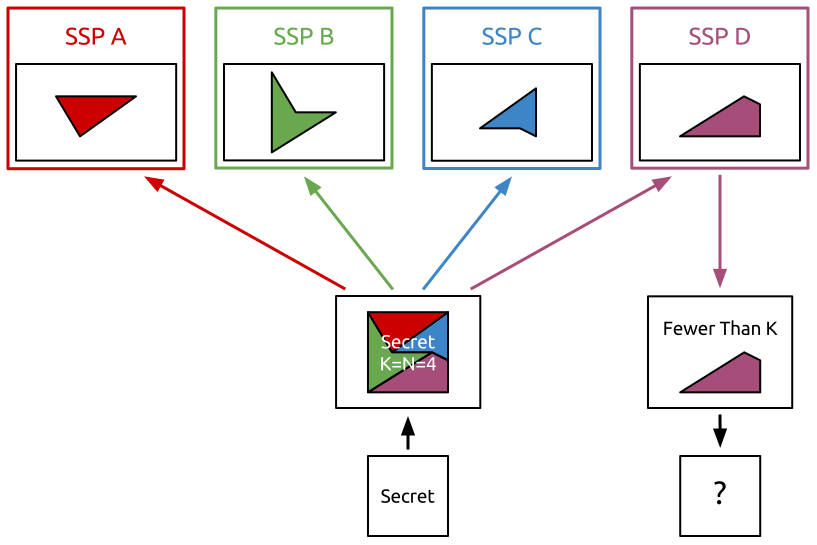
\includegraphics[height=200px]{./figs/out/Arch-Sharded.pdf}
  \caption{Sharding Secrets Between Multiple Providers}
  \label{fig:ssaas-sharded}
\end{figure}

Nonetheless, it is best if users can avoid placing high degrees of
trust in any single third party, FP or SSP. Fortunately, there is a
viable alternative for avoiding placing a high degree of trust in an
single SSP, even in the raw-secret storage SSP use case: sharding a
single user secret across multiple SSPs. As shown in
Figure~\ref{fig:ssaas-sharded} secure secret sharing systems such as
Shamir's $(k, n)$ threshold scheme~\cite{shamir1979} ensure that a
secret split into $n$ shares can not be reassembled using fewer than
$k$ shares in an unconditionally secure manner. Such schemes can be
applied in an SSaaS ecosystem to avoid affording (\emph{R}) and
(\emph{W}) capabilities to an SSP, even when storing raw user data. In
addition, secret sharing schemes have benefits related to redundancy
and data availability. Since $(k, n)$ threshold schemes include
redundant shares in any case where $n > k$, users can split their
secrets into $n$ shares stored with $n$ independent SSPs. Doing so
ensures that the user can recover their secret as long as at least $k$
SSPs remain operational and in possession of their designated
share. As such, sharding secrets, be they cryptographic keys or raw
data, across multiple SSPs is likely to become a standard
best-practice in SSaaS ecosystems for both the trust reduction and
increased reliability such a practice provides.

Even with secret sharding, users are still at risk of a successful
trust violation should multiple SSPs collude to betray a user's trust
(\emph{L}-type violation) or should multiple SSPs be compelled to turn
over shares of user secretes to a single entity (\emph{C}-type
violation). As such, user should select a set of SSPs across which to
shard our secrets that minimize \emph{L} and \emph{C} type violation
risk. Thus, in addition to the reputation-based selection criteria
outlined in \S~\ref{chap:ssaas:economics}, SSaaS user's should
consider several additional SSP selection criteria:

\begin{packed_desc}
\item[Geopolitical Diversity:] An ideal set of SSPs will be located
  across a range of non-cooperating geopolitical domains. This will
  greatly decrease the likelihood of a compelled (\emph{C}-type)
  violation by ensuring that no single entity has the ability to
  compel multiple SSPs to surrender user secret shares. See
  Chapter~\ref{chap:policy} for additional discussion of this point.
\item[Ownership Diversity:] Similarly, a user should only select SSPs
  owned and operated by independent entities. This decreases the
  likelihood of an (\emph{L}-type violation) by ensuring no single
  entity can instruct multiple SSPs to collude to reconstruct a user
  secret.
\end{packed_desc}

If the user shards their secrets across a diverse set of SSPs, all
with strong privacy-preserving reputations, they have a reasonable
likelihood of avoiding a successfully series of trust violations
resulting in the compromise of user privacy or security.

%%  LocalWords:  SSaaS SSPs FPs SSP HTTPS TBD SSaaS's SSP's FP HIPPA
%%  LocalWords:  Shamir's BitCoin FERPA PCI DSS Tutamen KSaaS
